\documentclass[12pt]{report}
\usepackage[utf8]{inputenc}
\usepackage{geometry}
\geometry{letterpaper, margin=0.25in}
\usepackage{graphicx} 
\usepackage{multicol}
\usepackage{parskip}
\usepackage{booktabs}
\usepackage{array} 
\usepackage{paralist} 
\usepackage{verbatim}
\usepackage{sectsty}
\usepackage[shortlabels]{enumitem}
\usepackage[ruled,vlined,linesnumbered]{algorithm2e}
\IncMargin{1.5em}

\usepackage{amsmath}
\usepackage{amssymb}
\usepackage{mathtools}
\usepackage{empheq}
\usepackage{xcolor}
\usepackage{bbm}
\usepackage{tikz}
\usepackage{pgfplots}
\usepackage{tikz-cd}
\usepackage{circuitikz}
\usepackage{multirow}
\pgfplotsset{compat=1.18}
\usetikzlibrary{intersections, decorations.markings}
\tikzset{
    marking along/.style n args={2}{
        decoration={
                markings, 
                mark=at position #1 with {\arrow{#2}}
        },
        postaction={decorate}
        },
    marking along/.default={0.5}{>}
    wavy/.style={
        decorate,decoration={coil,aspect=0}
     },
    two marks/.style n args={1}{
        decoration={
            markings,
            mark=at position 0.25 with {\arrow{#1}},
            mark=at position 0.75 with {\arrow{#1}}
         },
         postaction={decorate}
    }
    two marks/.default={>}
}

\colorlet{mygreen}{green!50!teal}
\colorlet{darkblue}{blue!60!black}

\newcommand{\ans}[1]{\boxed{\text{#1}}}
\newcommand{\vecs}[1]{\langle #1\rangle}
\renewcommand{\hat}[1]{\widehat{#1}}

\renewcommand{\P}{\mathbb{P}}
\newcommand{\R}{\mathbb{R}}
\newcommand{\E}{\mathbb{E}}
\newcommand{\Z}{\mathbb{Z}}
\newcommand{\N}{\mathbb{N}}
\newcommand{\Q}{\mathbb{Q}}
\newcommand{\C}{\mathbb{C}}

\newcommand{\ind}{\mathbbm{1}}
\newcommand{\qed}{\quad \blacksquare}

\newcommand{\brak}[1]{\left\langle #1 \right\rangle}
\newcommand{\bra}[1]{\left\langle #1 \right\vert}
\newcommand{\ket}[1]{\left\vert #1 \right\rangle}

\newcommand{\abs}[1]{\left\vert #1 \right\vert}
\newcommand{\mfX}{\mathfrak{X}}
\newcommand{\ep}{\varepsilon}

\newcommand{\Ec}{\mathcal{E}}
\newcommand{\Nc}{\mathcal{N}}
\newcommand{\A}{\mathcal{A}}
\newcommand{\F}{\mathcal{F}}
\newcommand{\Cc}{\mathcal{C}}
\newcommand{\B}{\mathcal{B}}
\newcommand{\M}{\mathcal{M}}
\newcommand{\X}{\chi}
\renewcommand{\L}{\mathcal{L}}

\newcommand{\sub}{\subseteq}
\newcommand{\st}{\text{ s.t. }}
\newcommand{\card}{\text{card }}
\renewcommand{\div}{\vspace*{10pt}\hrule\vspace*{10pt}}
\newcommand{\surj}{\twoheadrightarrow}
\newcommand{\inj}{\hookrightarrow}
\newcommand{\biject}{\hookrightarrow \hspace{-8pt} \rightarrow}
\renewcommand{\bar}[1]{\overline{#1}}
\newcommand{\overcirc}[1]{\overset{\circ}{#1}}
\newcommand{\diam}{\text{diam }}
\newcommand{\iid}{\overset{	ext{iid}}{\sim}}

\renewcommand{\Re}{\text{Re}\,}
\renewcommand{\Im}{\text{Im}\,}
\newcommand{\Var}{\text{Var}\,}
\newcommand{\Cov}{\text{Cov}\,}

\renewcommand{\tt}[1]{\texttt{#1}}

\DeclareMathOperator*{\argmax}{\arg\max}
\DeclareMathOperator*{\argmin}{\arg\min}

\newcommand{\sign}{\text{sign}\,}

\newcommand*{\tbf}[1]{\ifmmode\mathbf{#1}\else\textbf{#1}\fi}

\usepackage{tcolorbox}
\tcbuselibrary{breakable, skins}
\tcbset{enhanced}
\newenvironment*{tbox}[2][gray]{
    \begin{tcolorbox}[
        parbox=false,
        colback=#1!5!white,
        colframe=#1!75!black,
        breakable,
        title={#2}
    ]}
    {\end{tcolorbox}}

\newenvironment*{exercise}[1][red]{
    \begin{tcolorbox}[
        parbox=false,
        colback=#1!5!white,
        colframe=#1!75!black,
        breakable
    ]}
    {\end{tcolorbox}}

\newenvironment*{proof}[1][blue]{
\begin{tcolorbox}[
    parbox=false,
    colback=#1!5!white,
    colframe=#1!75!black,
    breakable
]}
{\end{tcolorbox}}
\newenvironment*{proposition}[1][gray]{
    \begin{tcolorbox}[
        parbox=false,
        colback=#1!5!white,
        colframe=#1!75!black,
        breakable
    ]}
    {\end{tcolorbox}}




\title{CSCI 2540: Advanced Probabilistic Methods in Computer Science}
\author{Milan Capoor}
\date{Fall 2026}
\begin{document}
\maketitle

\section{Sept 10}
\tbf{Why Probabilistic Methods?}
\begin{itemize}
    \item Randomized algorithms (hashing, quicksort, open key cryptography, finance, weather)
    \item Probabilistic analysis of algorithms (average case analysis, smoothed analysis)
    \item Modeling data (statistical ML)
\end{itemize}

\tbf{Course Topics:}
\begin{enumerate}
    \item Basic randomized algorithms and probabilistic analysis
    \item Large deviation bounds (Chernoff and Hoeffding bounds)
    \item The probabilistic method
    \item Martingale (in discrete space)
    \item Sample complexity and statistical learning theory
    \item Monte Carlo methods
    \item Converge of Monte Carlo Markov Chains
\end{enumerate}

\tbf{Example (Verifying Matrix Multiplication):} Suppose you have three $n\times n$ matrices $A, B, C$ in a boolean field. We want to verify $AB = C$. 

A naive matrix multiplication algorithm takes $\Theta(n^3)$ time ($\Theta(n^{2.37})$ at the absolute best). But we would hope verification can be done faster.

\begin{algorithm}
    \caption{Freivalds' Randomized algorithm in $\Theta(n^2)$}
        Choose a random vector $r \in \{0, 1\}^n$ uniformly at random.

        Compute $Br$ and $A(Br)$ 

        Compute $Cr$

        If $A(Br) \neq Cr$, return ``$AB \neq C$''. Otherwise, return ``$AB = C$''.
\end{algorithm}

\begin{tbox}{ \textbf{Theorem:} If $AB \neq C$ and $r$ is chosen uniformly at random from $\{0, 1\}^n$, then
    \[\P(ABr = Cr) \leq \frac{1}{2}\]}
    \emph{Proof:} 

    Take the case $AB \neq C$. Let $D = AB - C \neq 0$. Then 
    \[ABr = Cr \implies Dr = 0\]

    Since $D \neq 0$, there exists some $d_{ij} \in D \neq 0$. By definition of matrix multiplication, we have
    \[\sum_{j=1}^{n} d_{1j} r_j = 0 \iff r_1 = -\frac{1}{d_{11}} \sum_{j=2}^{n} d_{1j} r_j\]
    (assuming WLOG $d_{11} \neq 0$). 

    Letting $a_{1}, \dots, a_n$ being the values chosen at random from the set of variables $\{r_1, \dots, r_n\}$, we have 
    \[\P\left(r_1 = -\frac{1}{d_{11}} \sum_{j=2}^{n} d_{1j} a_j\right) \leq \frac{1}{2}\]
\end{tbox}
Hence, if $AB = C$ the algorithm is always correct. If $AB \neq C$ the algorithm is correct with probability at least $1/2$. We can repeat the algorithm $k$ times to reduce the error probability to $1/2^k$.

\tbf{Probability space:} ($\Omega, \F, \P)$ for $\Omega$ a sample space of outcomes, $\F$ a $\sigma$-algebra of allowable events (subsets of $\Omega$), and $\P: \F \to [0, 1]$ a probability measure.

In a \tbf{discrete probability space}, $\omega \in \Omega$ is a simple event and $\F = 2^{\Omega}$. 

\tbf{Probability function:} a function $\P: \F \to \R$ that satisfies 
\begin{enumerate}
    \item For all $E \sub \F$, $0\leq \P(E) \leq 1$
    \item $\P(\Omega) = 1$
    \item For any countable collecction of pairwise mutually disjoint events $E_1, E_2, \dots \in \F$, we have
    \[\P\left(\bigcup_{i \geq 1} E_i\right) = \sum_{i \geq 1} \P(E_i)\]
\end{enumerate}

In a discrete space, each \emph{atomic event} has a finite probability and the probability of an event $E$ is given by the sum of the probabilities of the atomic events in $E$

Let's return to Freivald's algorithm, 

\begin{proposition}
\textbf{Lemma:} Choosing $r = (r_1, \dots, r_n) \in \{0, 1\}^n$ uniformly at random is equivalent to choosing each $r_i$ independently and uniformly at random from $\{0, 1\}$
\end{proposition}

Hence a more formal version of the earlier proof proceeds:
\begin{align}
    \P(ABr = Cr) &= \sum_{x_2, \dots, x_n} \P((ABr = Cr) \cap ((r_2, \dots, r_n) = (x_2, \dots, x_n))) \\
    &\leq \sum_{x_2, \dots, x_n} \P\left(\left[r_1 = -\frac{1}{d_{11}} \sum_{j=2}^{n} d_{1j} x_j\right] \cap ((r_2, \dots, r_n) = (x_2, \dots, x_n))\right) \\
    &= \sum_{x_2, \dots, x_n} \P\left(r_1 = -\frac{1}{d_{11}} \sum_{j=2}^{n} d_{1j} x_j\right) \P((r_2, \dots, r_n) = (x_2, \dots, x_n)) \\
    &\leq \sum_{x_2, \dots, x_n} \frac{1}{2} \P((r_2, \dots, r_n) = (x_2, \dots, x_n)) \\
    &= \frac{1}{2} 
\end{align}

\section{Sept 15}

\subsection{Deciding Polynomial Identity}
\tbf{Problem:} Verify that $P(x) \equiv Q(x)$ for two polynomials $P, Q$, i.e. $H(x) = P(x) - Q(x) \equiv 0$.

\emph{Example:} Check if 
\[(x + 1)(x - 2)(x + 3)(x- 4)(x + 5)(x-6) \equiv x^6 - 7x^3 + 25\]

\tbf{Notational remark:} we use $\equiv$ to denote polynomial identity and $=$ for numerical equality.

\begin{algorithm}
    \caption{Randomized Polynomial Identity}
        Choose $r \in [1, \dots, m]$ \; 

        If $H(r) = 0$ output ``$P \equiv Q$'' else output ``$P \not\equiv Q$''
\end{algorithm}

\begin{tbox}{\textbf{Theorem:} Assume that $H(x) \not\equiv 0$ and $\deg(H) \leq d$. Then if $r$ is chosen uniformly at random from $\{1, \dots, m\}$, we have
\[\P(H(r) = 0) \leq \frac{d}{m}\]}
    \emph{Proof:} A polynomial of degree $d$ has at most $d$ roots. Hence, if $H(x) \not\equiv 0$, then there are at most $d$ values of $r$ such that $H(r) = 0$. Since $r$ is chosen uniformly at random from $\{1, \dots, m\}$, we have
    \[\P(H(r) = 0) \leq \frac{d}{m}\]
\end{tbox}

What about multivariate polynomials? 

\emph{Example:} 
\[H(x, y, z, w) = x^5 y^3(z^3 - w^4) + x^3(z^5 - w^3)(x^2y^4 - w^2) \overset{?}{\equiv} 0\]

Define the degree of a multivariate polynomial $H(x_1, \dots, x_n)$ as the maximum sum of the degrees in each of its monomials. For example, the degree of $H(x, y, z, w)$ above is $3+5+2+4 = 14$.

For this setting, no efficient deterministic algorithm is known. A polynomial with $n$ variables and degree $d$ can have up to $\binom{n+d}{d}$ monomials, which is exponential in $n$ 

\begin{tbox}{\textbf{Theorem (Schwartz-Zippel):}  Assume that $H(x_1, \dots, x_n) \not\equiv 0$ and $\deg(H) \leq d$. Then if $r_1, \dots, r_n$ are chosen independently and uniformly at random from a set $S$ (equivalently, sampling $(r_1, \dots, r_n)$ from $S^n$), then 
    \[\P(H(r_1, \dots, r_n) = 0) \leq \frac{d}{\abs{S}} \] }
    \emph{Proof:} By induction on $n$. 

    For $n = 1$, $H$ has at most $d$ roots and by the theorem above, 
    \[\P(H(r_1) = 0) \leq \frac{d}{\abs{S}}\]

    For $n > 1$, $H$ can be written as a polynomial in $x_n$ with coefficients that are polynomials in $x_1, \dots, x_{n-1}$:
    \[H(x_1, \dots, x_n) = \sum_{i \geq 0} x_n^i f_i(x_1, \dots, x_{n-1})\]

    Let $k \leq d$ be the largest index for which $f_k \not\equiv 0$. Then $\deg(f_k) \leq d - k$ and by the induction hypothesis,
    \[\P(f_k(r_1, \dots, r_{n-1}) = 0) \leq \frac{d - k}{\abs{S}}\]

    If $f_k(r_1, \dots, r_{n-1}) \neq 0$, then $H(r_1, \dots, r_{n-1}, x_n)$ is a nonzero univariate polynomial in $r_n$ of degree $k$. Hence by the univariate case,
    \[\P[H(r_1, \dots, r_n) = 0 \; | \; f_k(r_1, \dots, r_{n-1} \neq 0)] \leq \frac{k}{\abs S}\]

    Then since 
    \begin{align*}
        \P(A) &= \P(A \cap B) + \P(A \cap B^c)\\
        &= \P(A \; | \; B) \P(B) + \P(A \; | \; B^c) \P(B^c)\\
        &\leq \P(A \; | \; B) + \P(B^c)
    \end{align*}
    we have
    \begin{align*}
        \P(H(r_1, \dots, r_n) = 0) &= \P[H(r_1, \dots, r_n) = 0 \; | \; f_k(r_1, \dots, r_{n-1} \neq 0)] + \P[f_k(r_1, \dots, r_{n-1}) = 0]\\ 
        &\leq  \frac{k}{\abs{S}} + \frac{d - k}{\abs{S}} \\ 
        &= \frac{d}{\abs{S}}
    \end{align*}
    
\end{tbox}

Recall the definition of conditional probability.   

\textbf{Conditional Probability:} 
\[\P(E_1 \; | \; E_2) = \frac{\P(E_1 \cap E_2)}{\P(E_2)}\] 

where we can think of conditioning on $E_2$ as restricting the sample space to $E_2$. Hence, we have
\[\P(E_n) = \sum_{i=1}^{n} \P(E_n \; | \; E_i) \P(E_i)\]

This exposes a general method for the course: ``Suppose some nice condition holds and analyze the algorithm conditioned on that event. Then bound the probability of that event not holding.''

This theorem has a \tbf{one-sided error:} if $H \equiv 0$, the algorithm is always correct. If $H \not\equiv 0$, the algorithm is correct with probability at least $1 - d/\abs{S}$. We can repeat the algorithm $\ell$ independent times to reduce the error probability to $(d/\abs{S})^{\ell}$.

\textbf{Independent Events:} $E \perp F$ iff 
\[\P(E \cap F) = \P(E) \cdot \P(F)\] 

More generally, events $E_1, \dots, E_n$ are \tbf{mutually independent} iff for any subset $I \sub \{1, \dots, n\}$,
\[\P\left(\bigcap_{i \in I} E_i \right) = \prod_{i\in I} \P(E_i) \]

In particular, if $E \perp F$, then $\P(E \; | \; F) = \P(E)$. 

\section{Sept 17}

\tbf{Min-cut set:} a minimum set of edges that disconnects a graph.

Trivially, we can iterate over all nodes and cut all edges for the node with the minimum degree. This gives an upper bound on the size of the min-cut:
\[\text{min-cut} \leq \min_{v \in V} \deg(v)\]

Consider, however, this graph:

\begin{center}
    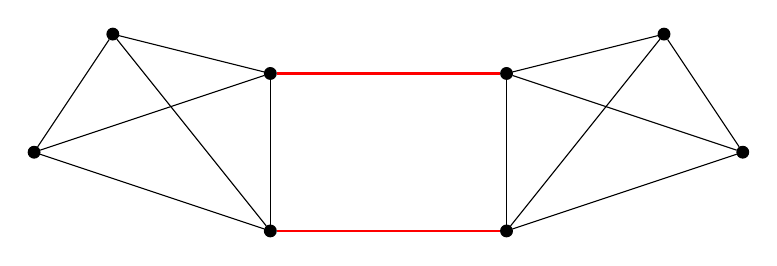
\begin{tikzpicture}[scale=1, every node/.style={circle,draw,fill=black,inner sep=1.5pt}]
    
      % Left cluster (K5 minus edge A1-A2)
      \node (A1) at (-2,1) {};
      \node (A2) at (-2,-1) {};
      \node (A3) at (-4,1.5) {};
      \node (A4) at (-5,0) {};
    
      % Right cluster (K5 minus edge B1-B2)
      \node (B1) at (1,1) {};
      \node (B2) at (1,-1) {};
      \node (B3) at (3,1.5) {};
      \node (B4) at (4,0) {};
    
      % Left K5 minus (A1,A2)
      \foreach \i/\j in {A1/A3,A1/A4,A2/A3,A2/A4,A3/A4, A1/A2}
        \draw (\i) -- (\j);
    
      % Right K5 minus (B1,B2)
      \foreach \i/\j in {B1/B3,B1/B4,B2/B3,B2/B4,B3/B4, B1/B2}
        \draw (\i) -- (\j);
    
      % The 2-edge cut connecting the two halves
      \draw[thick,red] (A1) -- (B1);
      \draw[thick,red] (A2) -- (B2);
    
    \end{tikzpicture}
\end{center}

Every node has degree 4, but the min-cut is 2.

As we will see, this is a deep problem with many applications. This problem happens to have a deterministic polynomial time algorithm related to max-flow but it is complicated and involves an $O(\abs{V}^2)$ algorithm run between every pair of nodes ($O(\binom{\abs{V}}{2})$ pairs).

\begin{algorithm}
    \caption{Randomized Min-cut Algorithm}
    \For{i=1:n-2}{

        Pick an edge uniformly at random\; 

        Contract the two vertices connected by that edge, elimate all edges connecting the two vertices\;
    }

    Output the set of edges connecting the two remaining vertices\;

\end{algorithm}

\begin{center}
    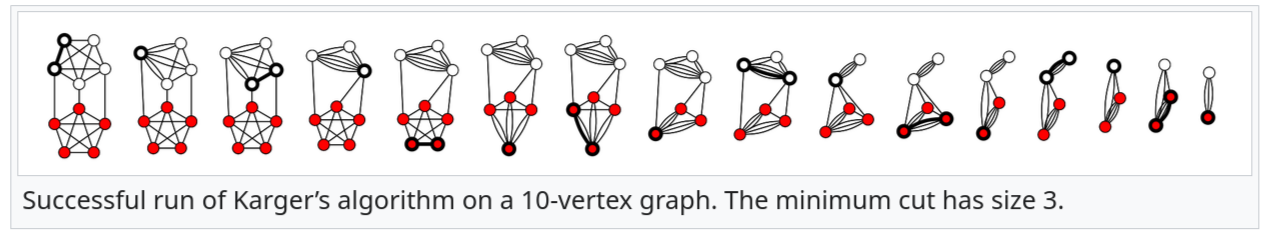
\includegraphics[width=\textwidth]{Images/mincut.png}
\end{center}

Notice that this algorithm fails precisely when we contract an edge in the min-cut. Following the strategy we saw last time, we would like to find the condition that makes the algorithm fail deterministically and then bound the probability of that condition holding.

\begin{tbox}{\textbf{Theorem:} 
    \begin{enumerate}
        \item The algorithm outputs a min-cut edge-set with probability 
        \[\geq \frac{2}{n(n-1)}\]
        \item The smallest set output in $O(n^2 \log n)$ iterations of the algorithm gives a correct answer with probability $1 - 1/n^2$.
        \end{enumerate}}
    \emph{Proof:} Assume the graph has a min-cut set of $k$ edges. We compute the probability of finding one particular such set $C$.

    Trivially, 
    \[\P(\text{alg. returns any min-cut}) \geq \P(\text{alg. returns min-cut } C)\]

    \begin{proposition}
        \textbf{Lemma:} If no edge of $C$ was contracted, the algorithm outputs $C$. 
    \end{proposition}

    First, notice that if no edge of $C$ was contracted, no edge of $C$ was eliminated. To see this, let $X$ and $Y$ be the two sets of vertices connected by edges in $C$. If no edge of $C$ was contracted, then no vertex in $X$ was contracted with a vertex in $Y$. Hence, all edges in $C$ remain in the graph and are output by the algorithm.

    As a corollary, if the algorithm terminates before contracting any edge in $C$, it gives the correct answer. 

    Finally, to show the one-sided error property, notice that vertex contraction does not reduce the size of the min-cut set but does reduce the size of the original graph. Intuitively, contracting an edge \emph{reduces the size of the sample space}

    \begin{proposition}
        \textbf{Lemma:} 
        \[\P(\text{no edge in } C \text{ is contracted}) \geq \frac{2}{n(n-1)}\]
    \end{proposition}

    Let $E_i$ be the event ``no edge contracted in iteration $i$ is in $C$'' so 
    \[F_i = \bigcap_{j=1}^i E_j = ``\text{no edge of } C \text{ is contracted in the first } i \text{ iterations}''\]
    
    Since the min-cut set has $k$ edges, all vertices have degree $\geq k$ (else the min-cut set would be smaller). Hence, the number of edges in the graph $ \geq nk/2$. 

    \[\P(E_1) = \P(F_1) = 1 - \frac{2k}{nk} =  1 - \frac{2}{n}\]

    Conditioning on $E_1$, after the first contraction, we have $n-1$ vertices and $k(n-1)/2$ edges but still $k$ edges in the min-cut set. By analogous argument,
    \begin{align*}
        \P(E_2) &= \P(E_2 \; | \; E_1) \cdot \P(E_1) + \P(E_2 \; | \;\bar E_1) \cdot \P(\bar E_1)\\ 
        \P(E_2 \; | \; E_1) &\geq 1 - \frac{k}{\abs{G_1}} \qquad (\text{where } \abs{G_1} = \# \text{ edges after iter 1} )\\ 
        &\geq 1 - \frac{k}{(n-1)k/2}\\ 
        &= 1 - \frac{2}{n-1}
    \end{align*}
    
    Of course, since $\P(E_1) = \P(F_1)$, 
    \[\P(E_2 \; | \; F_1) = \P(E_2 \; | \; E_1) \geq 1 - \frac{k}{k(n-1)/2} \geq 1 - \frac{2}{n-1}\]

    Inductively, 
   \begin{align*}
     \P(E_i \; | \; F_{i-1}) &= \P\left(E_i \; \big| \; \bigcap_{j=1}^{i-1} E_j\right)\\ 
     &\geq  1 - \frac{k}{k(n - i+1)/2}\\ 
     &= 1 - \frac{2}{n - i + 1}
   \end{align*}
   
    How do we compute $F_{n-1}$ given a sequence of $\P(E_i \; | \; F_{i-1})$? By chain rule:
    \begin{align*}
        \P(F_{n}) &= \P\left(\bigcap_{j=1}^{n} E_j\right)\\ 
        &= \P(E_{n-1} \; | \; F_{n-1}) \cdot \P(F_{n-1})\\ 
        &= \P(E_n \; | \; F_{n-1})\cdot \P(E_{n-1} \; | \; F_{n-2}) \cdots \P(E_2 \; | \; F_1) \cdot \P(E_1)
    \end{align*}
    
    We are interested in $\P(F_{n-2})$ since the algorithm terminates after $n-2$ iterations. Simply plugging in, 
    \begin{align*}
        \P(F_{n-2}) &= \P(F_1) \cdot \prod_{j=2}^{n-2} \P(E_j \; | \; F_{j-1})\\ 
        &\geq \prod_{i=1}^{n-2} \left(1 - \frac{2}{n - i + 1}\right)\\ 
        &= \prod_{i=1}^{n-2} \frac{n - i - 1}{n - i + 1}\\ 
        &= \frac{n - 2}{n} \cdot \frac{n - 3}{n - 1} \cdot \frac{n-4}{n-2} \cdots \cdot \frac{2}{n-1} \\ 
        &= \frac{2}{n(n-1)} \qed
    \end{align*}

    \div 

    \emph{Proof of Part 2:} Assume that we run the algorithm $n(n-1)\log n$ times and output the minimum cut set found across the iterations. We claim the probability of not finding a min-cut set is at most $1/n^2$.

    From the lemma proving the one-sided error, the output cannot be smaller than the min-cut set. Hence, the probability that $C$ is \emph{not} the output of any of the $n(n-1)\log n$ independent iterations is 
    \[\leq \left(1 - \frac{2}{n(n-1)}\right)^{n(n-1)\log n} \leq e^{-2\log n} =\frac{1}{n^2} \]

    Via Taylor Series, 
    \[e^{-x} = 1 - x + \frac{x^2}{2!} - \frac{x^3}{3!} + \cdots\]

    So for $x < 1$, 
    \[1 - x \leq e^{-x}\]

    
\end{tbox}

Once again, we can repeat this algorithm to reduce the error because it has \tbf{one-sided error} (the algorithm is completely correct for one specific outcome while bounding the error probability for the other outcome)

\section{Sept 22}

\begin{algorithm}
    \caption{Quicksort}
    \tbf{Input:} An array $S$

    \tbf{Output:} The array $S$ in sorted order.

    Choose an element $y \in S$

    Compare all elements of $S$ to $y$. Let 
    \begin{align*}
        S_1 &= \{x \in S - \{y\} \; | \; x \leq y\}\\ 
        S_2 &= \{x \in S- \{y\} \; | \; x > y\}
    \end{align*}

    Return $\tt{Quicksort}(S_1) \cup \{y\} \cup \tt{Quicksort}(S_2)$

\end{algorithm}

What can we say about the run time of this algorithm? Well, it depends on what it means to ``choose an element $y \in S$''. 

In the \emph{randomized} version of the algorithm, we choose $y$ uniformly at random from $S$. 

But if we were to choose $y$ deterministically (say splitting the array in half), we could end up with a worst case run time of $O(n^2)$ or else do well and get $O(n \log n)$ run time.

Let $T(n)$ be the number of comparisons made by the algorithm on an array of size $n$. 

Here, $T(n)$ is a \emph{random variable}.

\textbf{Random Variable:} $X$ is a random variable if it is a function $X: \Omega \to \R$ from the sample space $\Omega$ to the real numbers.

\tbf{Random Vector:} $X^d: \Omega \to \R^d$

\tbf{Discrete random variable:} a random variable that takes on only a finite or countably infinite number of values. In this case, we use notation 
\[\P(X = a) = \P(\{s \in \Omega: X(s) = a\}) = \sum_{s \in \Omega: X(s) = a} \P(s)\]

Viewing random variables as functions of events, we can generalize the definition of independence to random variables: 

\tbf{Independent Random Variables:} $X \perp Y$ iff for all $x, y \in \Omega$,
\[\P(X = x \land Y= y) = \P(X = x) \cdot \P(Y = y)\]

Similarly, $X_1,\, \dots,\, X_n$ are\tbf{ mutually independent} iff for all $a_1, \dots, a_n \in \R$,
\[\P(X_1 = a_1 \land \dots \land X_n = a_n) = \prod_{i=1}^{n} \P(X_i = a_i)\]

\tbf{Median:} the median(s) of a random variable is a value $m$ such that 
\[\begin{cases}
    \P(x < m) \leq \frac{1}{2}\\ 
    \P(X > m) < \frac{1}{2}
\end{cases}\]
for a symmetric distribution, the median is the same as the mean.

Finally, we can define the expectation of a random variable:
\[\E[X] = \sum_{i \in \text{range}(X)} i \cdot \P(X = i)\]
where $\E[X]$ exists iff $\sum_i \abs{i} \P(X = i) < \infty$ (i.e. the sum converges uniformly).

\begin{tbox}{\textbf{Theorem:} The expected number of steps in the randomized version of quicksort is
    \[\E[T(n)] = O(n \log n)\]}

    \emph{Proof:} Let $s_1, \dots, s_n$ be the sorted elements of $S$. For $i = 1:n$ and $j > i$, define 
    \[X_{i, j} = \begin{cases}
        1 & \text{if } s_i, s_j \text{ are compared in the algorithm} \\ 
        0 & \text{otherwise} \\
    \end{cases}\]
    (for example, after the first partition elements of $S_1$ are never compared to elements of $S_2$). Then
    \[T(n) = \sum_{i=1}^{n} \sum_{j>i} X_{i, j}\]

    By linearity of expectation,
    \[\E[T(n)] = \sum_{i=1}^{n} \sum_{j>i} \E[X_{i, j}]\]

    Since $X_{i, j}$ is a Bernoulli random variable, 
    \[\E[X_{i, j}] = 0\cdot \P(X_{i, j} = 0) + 1\cdot \P(X_{i, j} = 1) = \P(X_{i, j} = 1)\] 

    Notice that $s_i$ and $s_j$ are compared if and only if one of them is chosen as the pivot before any of the $j-i-1$ elements between them is chosen. 

    Since elements are chosen uniformly at random, $X_{i,j} = 1$ iff the first pivot chosen in the set is $\{s_i, s_{i+1}, \dots, s_j\}$ is either $s_i$ or $s_j$.

    \[\E[X_{i, j}] = \frac{2}{j-i+1}\]

    Substituting back into the expectation of $T(n)$, we have
    \begin{align*}
        \E[T(n)] &= \sum_{i=1}^{n} \sum_{j>i} \frac{2}{j-i+1}\\ 
        &\leq n \sum_{k=1}^{n} \frac{2}{k}\\
        &\leq 2nH_n\\ 
        &= 2n \log n + O(n)
    \end{align*}
    where $H_n$ is the harmonic series 
    \[H_n = \sum_{i=1}^n \frac{1}{i} \approx \int_1^n \frac{1}{x} dx = \log n\]

\end{tbox}

Notice in particular that this analysis did not require any knowledge of the distribution of the input array $S$.

\begin{exercise}
    \textbf{Exercise:} Prove 
    \begin{enumerate}
        \item $\E[X + Y] = \E[X] + \E[Y]$
        \item for $c \in \R$ and $X$ an RV, $\E[cX] = c\E[X]$    \end{enumerate}
\end{exercise}

\begin{exercise}
    \textbf{Exercise:} Prove $\log n \leq H_n \leq \log n + 1$
\end{exercise}

\begin{algorithm}
    \caption{Deterministic Quicksort}

    \tbf{Input:} An array $S$

    \tbf{Output:} The array $S$ in sorted order.

    Let $y$ be the first element in $S$

    Compare all elements of $S$ to $y$. Let 
    \begin{align*}
        S_1 &= \{x \in S - \{y\} \; | \; x \leq y\}\\ 
        S_2 &= \{x \in S- \{y\} \; | \; x > y\}
    \end{align*}

    Return $\tt{DetQuicksort}(S_1) \cup \{y\} \cup \tt{DetQuicksort}(S_2)$
\end{algorithm}

\begin{tbox}{\textbf{Theorem:} the expected run time of deterministic Quicksort on a random permutation of $S$ is $O(n \log n)$}
    \emph{Proof:} Set $X_{i, j}$ as before. If all permutations have equal probability, then permutations of $S_i, \dots, S_j$ have equal probability. 

    Again,
    \[\P(X_{i, j} = 1) = \frac{2}{j - i + 1}\]
    and 
    \[\E[T(n)] = \sum_{i=1}^{n} \sum_{j>i} \frac{2}{j - i + 1} = O(n \log n)\]
\end{tbox}

This opens the way for two classifications of uses of randomness in algorithms:
\begin{enumerate}
    \item \tbf{Randomized algorithm:} algorithms where the analysis is true for all inputs, repeated runs are independent, and the sample space is the space of random choices made by the algorithm.
    \item \tbf{Probabilistic Analysis of algorithms:} The sample space is the space of all possible inputs; If the algorithm is deterministic repeated runs give the same output.
\end{enumerate}

In particular we will be interested in:
\begin{enumerate}
    \item \tbf{Monte Carlo Algorithm}: a randomized algorithm that may produce an incorrect solution.
    \item \tbf{Las Vegas algorithm:} a randomized algorithm that always produces the correct output.
\end{enumerate}

For decision problems: A \emph{one-side error Monte Carlo algorithm} errs only one one possible output, otherwise it is a two-side error algorithm.

In both types of algorithms the run-time is a random variable.

\tbf{The Random Allocations Paradigm:} set of algorithms where we randomly allocate $m$ balls into $n$ bins.
\begin{itemize}
    \item Used for load balancing, hashing, routing, distributed computing, and more
\end{itemize}

\begin{algorithm}
    \caption{The Coupon Collector Problem}

    \tbf{Input:} $n$ bins

    \tbf{Output:} The number of balls placed until every bin has at least one ball.

    Place balls independently and uniformly at random into $n$ bins. 
    
    Continue until every bin has at least one ball. Let $X$ be the number of balls placed.
\end{algorithm}

\begin{tbox}{\textbf{Theorem:} 
    \begin{enumerate}
        \item $\E[X] = nH_n = n \log n + \Theta(n)$
        \item $\P(X \geq 2H_n) = \Theta(1/n)$
    \end{enumerate}}

    Let $X_i$ be the number of balls placed when there were $i - 1$ non-empty bins. Then 
    \[X = \sum_{i=1}^n X_i\] 
    so $X_i$ is the number of trials until we hit an empty box, that is: $X_i$ is a geometric random variable with success probability 
    \[p_i = 1 - \frac{i - 1}{n}\]

    \emph{Proof:} 
\end{tbox}

\tbf{Geometric random variable:} $X$ is a geometric random variable with success probability $p$ on $n = 1,2,\dots$ 
\[\P(X =n) = (1-p)^{n-1} p\]

(Commonly used for the number of trials until the first success in a sequence of independent Bernoulli trials.)

\begin{tbox}{\textbf{Lemma (Memoryless Distribution):} For a geometric random variable $X$ with success probability $p$,
    \[\P(X = n + k \; | \; X > k) = \P(X = n)\]}
    \emph{Proof:} 
    \begin{align*}
        \P(X = n + k \; | \; X > k) &= \frac{\P(X = n + k \land X > k)}{\P(X > k)}\\
        &= \frac{\P(X = n + k)}{\P(X > k)}\\
        &= \frac{(1-p)^{n+k-1}p}{\sum_{i=k}^{\infty} (1-p)^i p}\\ 
        &= \frac{(1-p)^{n+k-1}p}{(1-p)^k}\\
        &= (1-p)^{n-1}p\\
        &= \P(X = n)
    \end{align*}
\end{tbox}

Note that the geometric distribution is the only discrete memoryless distribution (and the exponential distribution is the only continuous memoryless distribution).

\begin{exercise}
    \textbf{Exercise:} Prove that the expectation of $X \sim G(p)$ is 
    \[\E[X] = \sum_{i \geq 1} i (1-p)^{i-1} p = \frac{1}{p}\]
\end{exercise}

\tbf{Conditional Expectations:}
\[\E[Y \; | \; Z= z] = \sum_y y P(Y= y \; | \; Z = z)\]

\begin{tbox}{\textbf{Lemma:} For any random variables $X, Y$
    \[\E[X] = \E_Y[E_X[X \; | \; Y]] = \sum_y \P(Y = y) \E[X \; | \; Y = y]\]}
    \emph{Proof:} 

    \begin{align*}
        \E_Y[E_X[X \; | \; Y]] &= \sum_y \P(Y = y) \E[X \; | \; Y = y]\\
        &= \sum_y \P(Y = y) \sum_x x P(X = x \; | \; Y = y)\\
        &= \sum_y \P(Y = y) \sum_x x \frac{\P(X = x, Y = y)}{\P(Y = y)}\\
        &= \sum_y  \sum_x x P(X = x, Y = y)\\
        &= \sum_x x P(X = x)\\
        &= E[X]
    \end{align*}
\end{tbox}

This gives us an easier way to compute the expectation of $X \sim G(p)$: 

\begin{tbox}{\textbf{Proposition:} Let $X \sim G(p)$ be a geometric random variable with success probability $p$. Then
    \[\E[X] = \frac{1}{p}\]}
    \emph{Proof:} 

    Let $Y = 1$ if the first trial is a success and $Y = 0$ otherwise. Then
    \begin{align*}
        \E[X] &= \P(Y = 0) \E[X \; | \; Y = 0] + \P(Y = 1) \E[X \; | \; Y = 1]\\
        &= (1-p) \E[X \; | \; Y = 0] + p \E[X \; | \; Y = 1]\\
    \end{align*}

    Trivially, $\E[X \; | \; Y = 1] = 1$. In the case $Y = 0$, let $Z$ be the number of trials until the first success after the first trial. 

    By the memoryless property, $Z \sim G(p)$ and $\E[Z] = \E[X]$. Hence,
    \[\E[X] = (1 - p) \E[Z + 1] + p = (1- p) \E[Z] + 1 \implies \E[X] = \frac{1}{p}\]
\end{tbox}

\end{document}